\section{Systemmodel}
	\subsection{System structure}
			\subsubsection{Modules}
				%INSERT SYSTEMMODELCHART HERE
				The main architecture pattern the system is oriented to, is the Model-View-Controller. But 				only the main structure, the architecture should be seen as parallel model.
			\subsubsection{Controller}
				The Controller is basically the whole scheduler-module. It controls the data flow with the 				data structure(Model) and the Data Mining-module which both of them are part of the 						scheduler. Furthermore, the scheduler is responsible for the communication with the code-             				and executer interface and the MPI-world. There will be a scientific code bound to the 						scheduler and executed with different tasks(different parameter input), those will be 						brought in order through the scheduler. This will be organized with special scheduler 						algorithms depend on the data mining and the statistics
			\subsubsection{Model}
				The Model is represented as an high performance file system. Data which will be collected 					for statistics will be stored in such a file in the file system. Also the data for 							bookkeeping with information about the progress of the tasks which are executed on the 						computer cluster will be stored in one file. The queue of the task order will be also 						placed in a file. 
			\subsubsection{View}
				The essential point of visualization will be the graphical output of the collected data. 					Bookkeeping and statistic can be plotted after the calculation.
				A GUI is a nice-to-have feature and is first of all not in planning. The input for the 						controller will be managed trough the MOAB Interface.

\subsection{Scenarios}
			%szenario
\subsection{Use cases}

	\begin{figure}
		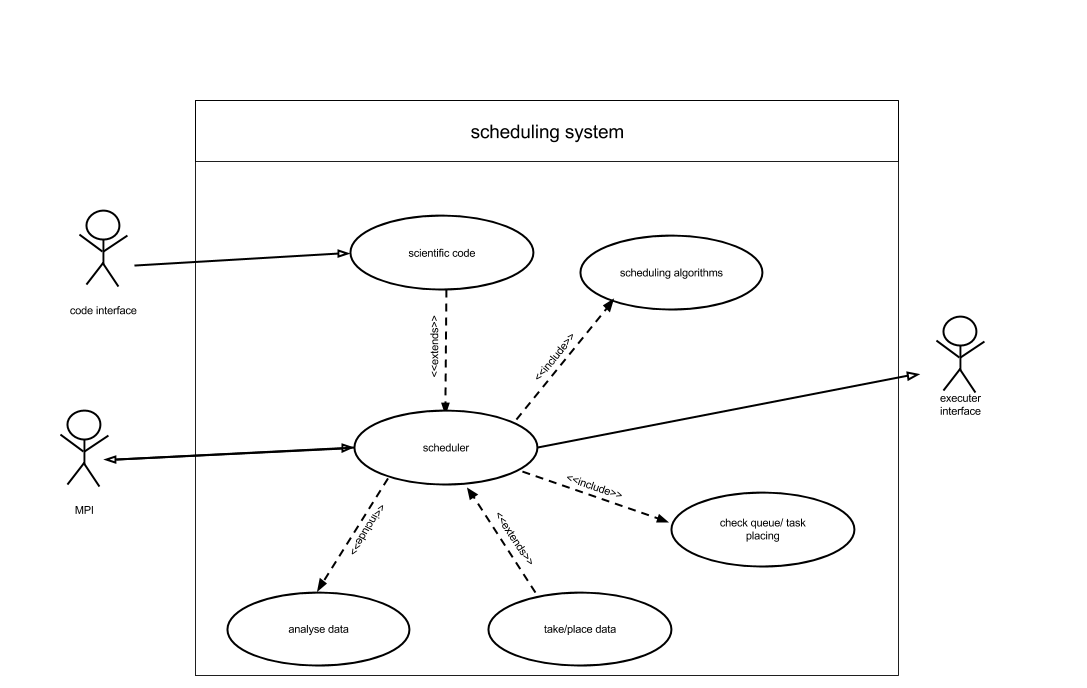
\includegraphics[width=1.5\textwidth,scale=0.75,trim=7cm 0 -7cm 0]{images/usecasediagram.png}
		\caption{Activity diagram}
	\end{figure}

\title{Task Stealing (Nice to have)}

\begin{enumerate}[1. ]


\item Brief Description
\newline
This use case describes the way a task stealing algorithm works inside a dynamic scheduler in order to reduce the amount of process migration between processors.

\item Actors
\newline
No actors. 


\item Preconditions
\begin{enumerate}
\item The scheduler has been initialized and it has already created a MPI memory window for RMA (Remote Memory Access).
\item Information about initial tasks has been collected from code preprocessing, received tasks from which have been placed to the queue.
\end{enumerate}

\item Basic Flow of Event
\newline
The use case begins when the scheduler checks if there are tasks in its own queue.If there is a task in the queue, it will be executed. After the task has been executed, all collected results will get placed in the database in an organized manner.
If there isn't any task in the queue, the task stealing process will be initiated. First of all, the scheduler will cycle through all running processes in other processors and try to steal an idle task from them. In order to check the other processes' queue for an idle task, the scheduler tries to block the RMA window for offsets and statuses, after which it checks whether there are any idle tasks. If the queue is empty or if the RMA window is currently blocked, the scheduler repeats the same procedure for remaining processors. If after checking all processes, no idle task was found, the scheduler changes its own state to idle. If this idle state doesn't change for a specific amount of cycles, which means that no tasks were stolen in this period, the scheduler finally checks to make sure that no process is currently running in any processor and if that's the case, it finishes its own routine. 


\item Post-conditions
\begin{enumerate}
\item The scheduler frees the allocated MPI memory window for RMA.
\item The scheduler executes the finishing post processing routine, where it collects information from the whole process (e.g. global total run time).
\end{enumerate}

\item Special requirements

\begin{enumerate}
\item The scheduler should have access to the executer interface.
\item The scheduler should be accessible through an interface, in order to receive new tasks from the code interface.
\end{enumerate}

\end{enumerate}

\subsection{Object model}

\subsection{Dynamic models}

\subsection{Graphical user interface}
			maybe